\chapter{Praktická část}

%%%%%%%%%%%%%%%%%%%%%%%%%%%%%%%%%%%%%%%%%%%%%%%%%
\section{Analýza}

%TODO obrázek nějakého flow

% popis Manty
\subsection{Manta Flow}
\textit{Manta Flow}\footnote{https://getmanta.com/} je nástroj umožňující automatickou analýzu zdrojového kódu (SQL, Java) a následný popis transformační logiky v něm obsažené. Software je schopný rozpoznat i těžce čitelné konstruky zdrojového kódu. Díky tomu dokáže automaticky zanalyzovat rozsáhlé databáze a vytvořit z nich přehlednou mapu datových toků, neboli \textit{Data Lineage}. To se v praxi využívá převážně k optimalizaci datových skladů, snižování nákladů na vývoj softwaru, provádění dopadových analýz a při dokumentování prostředí pro potřeby regulačních úřadů.

Nástroj má dvě hlavní komponenty (viz diagram \ref{fig:ana-flow-comp}): 
\begin{itemize}
	\item{\textit{Manta Flow CLI}}: je Java řádková aplikace provádějící extrakci skriptů ze zdrojových databází a uložišť a jejich analýzu. Analyzovaná data jsou následně poslána \textit{Manta Flow Serveru}. \textit{Klientská aplikace} také může nahrávat vygenerované exporty ze \textit{serveru} do externí metadatové databáze. 
	\item{\textit{Manta Flow Server}}: je serverová Java aplikace, která ukládá získané informace do interního metadatového uložiště, transformuje je, umožňuje jejich visualizaci a přístup k nim pomocí veřejného API. 
\end{itemize}

Interakce mezi \textit{klientskou} a \textit{serverovou} částí aplikace je popsána zjednodušeným sekvenčním diagramem \ref{fig:ana-flow-seq}. Pro tuto práci je podstatná především \textit{serverová} část aplikace a její interakce s metadatovým uložištěm (kapitola \ref{sec:ana_components}). \textit{Klientská} část aplikace je proto popsána méně detailně (kapitola \ref{\label{sec:ana_other}}).

\begin{figure}
\begin{center}
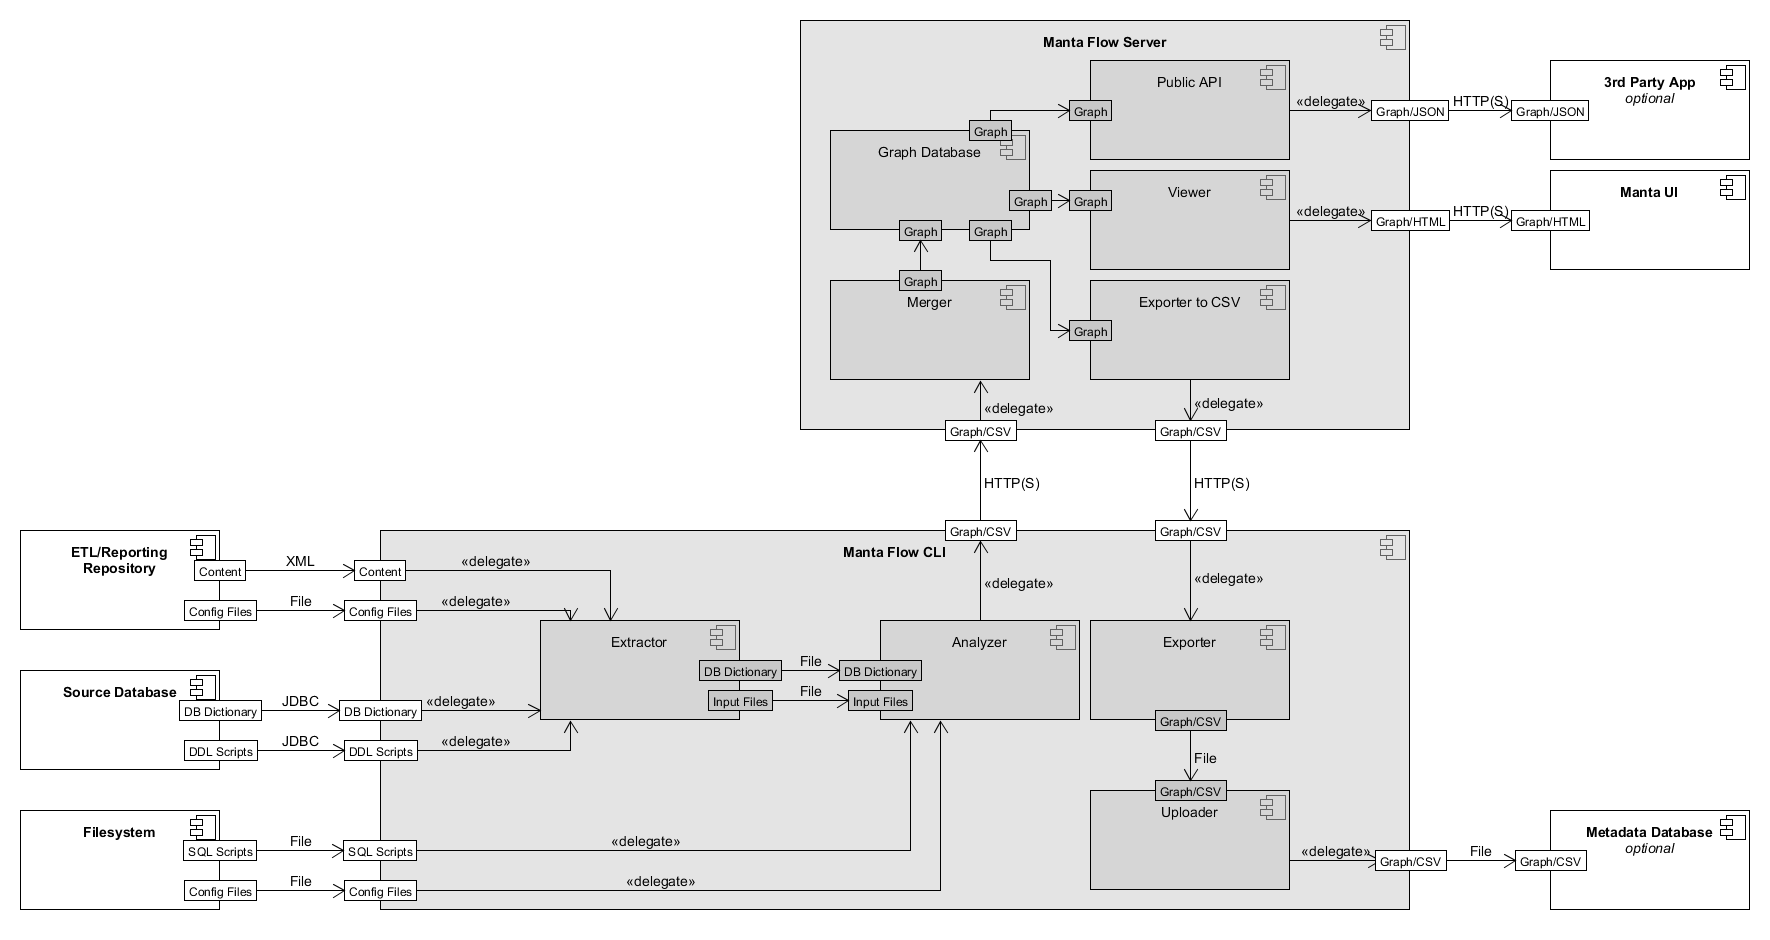
\includegraphics[width=14cm]{figures/flow_comp}
\caption{Architektura \textit{Manta Flow}}
\label{fig:ana-flow-comp}
\end{center}
\end{figure}

\begin{figure}
\begin{center}
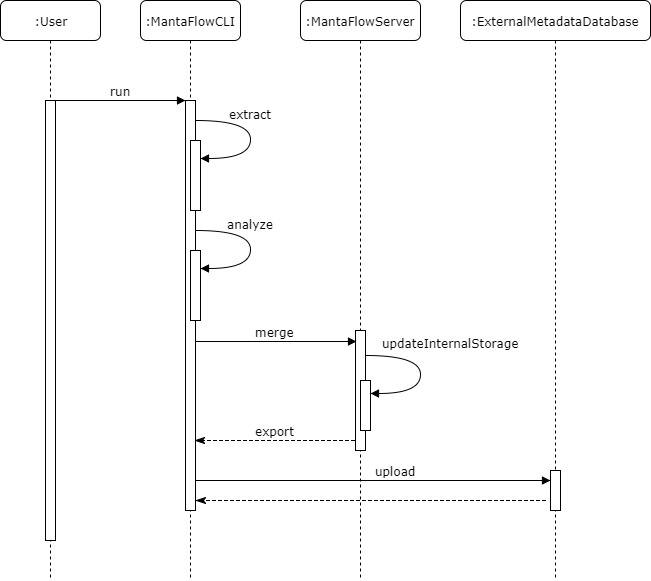
\includegraphics[width=14cm]{figures/flow_seq}
\caption{Interakce mezi \textit{klientskou} a \textit{serverovou} částí \textit{Manta Flow}}
\label{fig:ana-flow-seq}
\end{center}
\end{figure}


\subsection{Metadatové uložiště}
\label{sec:ana_model}
Jak již bylo zmíněno v úvodu práce (kapitola \ref{sec:uvod}) metadatové uložiště produktu \textit{Manta Flow} je aktuálně implementováno grafovou databází \textit{Titan} (ve verzi 0.4) a je snaha o výměnu této databáze\cite{Kovar18}. 
Než přistoupíme k bližšímu popisu jednotlivých komponent aplikace a jejich interakcí s metadatovým uložištěm (kapitola \ref{sec:ana_components}, je třeba nejdříve popsat entity, které jsou součástí analýzy datových toků a datový model metadatového uložiště (zobrazený na obrázku \ref{fig:ana-model}\footnote{Z modelu metadatového uložiště je zřejmé, že ne všechny podgrafy tvoří \textit{strom}. Vlastnosti \textit{stromu} nicméně porušují pouze hrany typu \textit{directFlow} a \textit{filterFlow}, které jsou výsledkem analýzy datových toků a jejichž odstraněním by strom vznikl. V textu je tak v některých případech používána teminologie vztahující se ke \textit{stromům} (například \textit{kořen}) - na celý graf je nahlíženo jako ne \textit{les}.}). 

% entity datového modelu
V procesu analýzy datových toků hraje roli mnoho entit z analyzovaných systémů. Ty se navíc mohou výrazně lišit systém od systému - \textit{Manta Flow} může analyzovat širokou škálu spolu propojených databázových systémů a integračních služeb. Obecně lze říci, že každý systém obsahuje zdroje a cíle dat (tabulky, soubory, ...) a transformace dat (skripty, \textit{\nomExpl{ETL}{Extract Load Transform}} workflow, procedury, makra a další).

\begin{figure}
\begin{center}
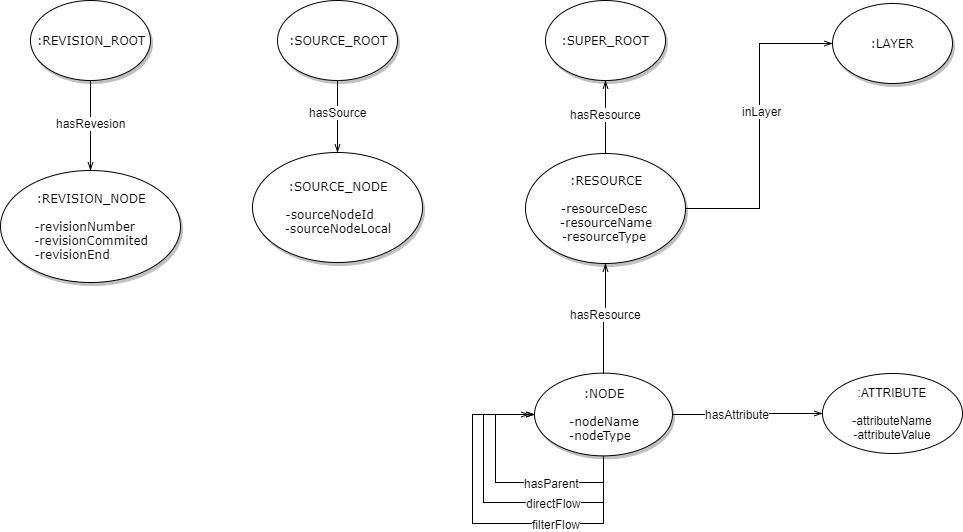
\includegraphics[width=14cm]{figures/model}
\caption{Model grafové databáze}
\label{fig:ana-model}
\end{center}
\end{figure}

% datový model
Samotný datový model se skládá z devíti typů uzlů:

\begin{itemize}
	\item{\textit{SUPER\_ROOT}}: Uzel (právě jeden v databázi), který slouží jako umělý kořen všech uzlů typu \textit{RESOURCE}. 
	\item{\textit{RESOURCE}}: Uzly tohoto typu reprezentují zdrojové systémy - zdroje definic objektů, zdrojových kódů, ETL řešení a další.  
	\item{\textit{NODE}}: Uzly typu \textit{NODE} představují reálné objekty zdrojového systému - databáze, tabulky, sloupce, procedury, skripty a další. 
	\item{\textit{LAYER}}: Uzly typu \textit{LAYER} reprezentují vrstvy modelu metadat. Datové toky nalezené při analýze zdrojových kódů jsou vždy ukládány do \textit{fyzické vrstvy}, ze které je potom možné generovat abstraktnější vrstvy modelu datových toků.  
	\item{\textit{ATTRIBUTE}}: Uzly typu \textit{ATTRIBUTE} reprezentují atributy uzlů typu \textit{NODE} - parametry sloupců, popisy databázových objektů a další.
	\item{\textit{SOURCE\_ROOT}}: Uzel (právě jeden v databázi), který slouží jako umělý kořen všech uzlů typu \textit{SOURCE\_NODE}. 
	\item{\textit{SOURCE\_NODE}}: Uzly typu \textit{SOURCE\_NODE} reprezentují soubory se zdrojovými kódy extrahovanými ze zdrojových systémů. 
	\item{\textit{REVISION\_ROOT}}: Uzel (právě jeden v databázi), který slouží jako umělý kořen všech uzlů typu \textit{REVISION\_NODE}. 
	\item{\textit{REVISION\_NODE}}: Uzly typu \textit{ATTRIBUTE} reprezentují revize modelu metadat, definují tedy jeho verzování. Kromě dalších parametrů mají všechny hrany grafu parametry \textit{tranEnd} a \textit{tranStart} definující platnost hran (viz obrázek \ref{fig:ana-model-rev}). Při každé analýze zdrojových systémů (která je prováděna dávkově klientskou částí aplikace) je vytvořena nová revize metadatového uložiště obsahující všechny objekty zdrojových systémů.\footnote{Je snaha tento princip upravit tak, aby byly objekty v metadatovém uložišti minimálně repklikovány \cite{Sykora17}.}  
\end{itemize}

 a osmi typů hran:

 \begin{itemize}
	\item{\textit{hasResource}}: Hrana přiřazuje objekty (uzly typu \textit{NODE}) ke svým zdrojovým systémům (uzlům typu \textit{RESOURCE}). Hrana je také použite k propojení uzlů typu \textit{RESOURCE} s uzlem \textit{RESOURCE\_ROOT}.
	\item{\textit{hasParent}}: Hrana mezi dvěmi uzly typu \textit{NODE} vytvářející klasickou hiearchickou strukturu mezi těmito uzly - strom závislostí objektů zdrojových systémů. 
	\item{\textit{directFlow}}: Hrana mezi dvěmi uzly typu \textit{NODE} říkající, že mezi těmito uzly existuje přímý datový tok (ve směru hrany).
	\item{\textit{filterFlow}}: Hrana mezi dvěmi uzly typu \textit{NODE} říkající, že mezi těmito uzly existuje nepřímý datový tok (ve směru hrany).
	\item{\textit{hasAttribute}}: Hrana přiřazující uzlům typu \textit{NODE} jejich atributy (uzly typu \textit{ATTRIBUTE}).
	\item{\textit{inLayer}}: Hrana typu \textit{inLayer} spojeju zdroje (uzly typu \textit{RESOURCE}) a vrstvy a říká, že zdroj patří do dané vrstvy modelu metadat. 
	\item{\textit{hasSource}}: Hrana je použita k propojení uzlů reprezentujících zdrojové kódy (uzly typu \textit{SOURCE\_NODE}) s uzlem \textit{SOURCE\_ROOT}.
	\item{\textit{hasRevision}}: Hrana je použita k propojení uzlů reprezentujících revize modelu metadat (uzly typu \textit{REVISION\_NODE}) s uzlem \textit{REVISION\_ROOT}.
\end{itemize}

\begin{figure}
\begin{center}
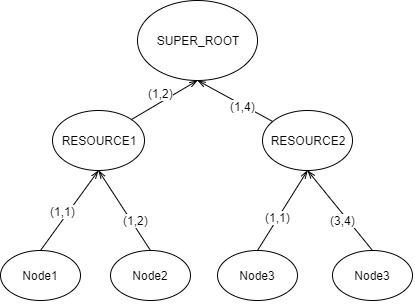
\includegraphics[width=6cm]{figures/model_revisions}
\caption{Způsob verzování modelu metadat}
\label{fig:ana-model-rev}
\end{center}
\end{figure}

Uzly i hrany mají dle svého typu několik specifických atributů, ty ale nebudeme blíže popisovat, protože nejsou pro analýzu zásadní. 

V metadatovém uložišti je dále definováno několik typů indexů, konkrétně se jedná o standardní indexy:

\begin{itemize}
	\item{\textit{indexy na kořeny}}: indexy pro konkrétní uzly, kořeny jednotlivých stromů datového modelu - \textit{SUPER\_ROOT, SOURCE\_ROOT, REVISION\_ROOT}
	\item{\textit{indexy na atributy hran}}: indexy zrychlující dohledávání atributů hran
	\item{\textit{indexy na typy hran}}: indexy zrychlující dohledávání hran daného typu pro jednotlivé uzly
\end{itemize}

a externí \textit{Apache Lucene} indexy, které slouží pro \textit{fulltextové} vyhledávání uzlů dle jejich názvů a pro intervalové vyhledání revizí. 


\subsection{Popis komponent serverové části}
\label{sec:ana_components}

Aplikace \textit{Manta Flow} praceje s metadatovým uložištěm několika různými způsoby, přičemž různé moduly aplikace využívají jeden či více těchto přístupů (a často také provádí vlastní pomocné dotazy přímo do metadatového uložiště). Cílem této sekce je tyto způsoby manipulace s metadatovým uložištěm identifikovat a popsat (není tedy účelem detailní technický popis všech dotazů do metadatového uložiště, ale spíše popis obecných principů a specifických situací - například netradiční zacházení s transakcemi). 

\subsubsection{Connector}
\label{sec:ana_connector}
Modul, který je nejblíže metadatovému uložišti, tzv. \textbf{connector} má dvě hlavní zodpovědnosti - zajištění připojení aplikace k uložišti a provádění dotazů nad ním. 

%Operations
Modul obsahuje sadu základních dotazů, tzv. \textit{operatinos}, mezi které patří například: 
\begin{itemize}
	\item{získání předka uzlu}
	\item{získání atributů uzlu}
	\item{získání sousedních uzlů a hran}
	\item{získání cesty ke kořeni}
	\item{získání podstromu}
\end{itemize} 
Tyto operace přímo přistupují do databáze a pomocí programovacího jazyka \textit{Gremlin}\footnote{Používá se \textit{TinkerPop} ve verzi \textit{2.6}.} a jsou na nich postaveny složitější operace nad grafouvou databází. U základních operací nejsou transakce řízeny explicitně, ale implicitně grafovou databází.

% Algorithm
Další částí modulu \textit{connector} jsou tzv. algoritmy, tedy komponenta, pomocí které jsou v metadatovém uložišti hledány samotné datové toky. Tato komponenta řetězí několik grafových algoritmů, přičemž první z nich získá z metadatového uložiště podmnožinu datových toků, která je dalšími algoritmy filtrována a omezována. Tímto způsobem vzniká tzv. \textit{referenční view} - objekt obsahující kompletní graf datových toků pro zadané výchozí uzly a směr datových toků. To je pak využ   íváno dalšími moduly aplikace, například \textit{viewerem} (viz \ref{sec:ana_viewer}), který dle parametrů zadaných ve webové aplikaci graf datových toků vizualizuje.
Jednotlivé algoritmy používají výše popsané základní operace (\textit{operations}) a v některých případech také samy dotazují metadatové uložiště přímo pomocí jazyka \textit{Gremlin}. 

% Traversal
Posledním způsobem manipulace s metadatovým uložištěm, který modul umožňuje je přístup pomocí \textit{traverserů}. Ty pracují na obecném principu \textit{traversování} grafů popsaném v kapitole \ref{sec:gdb-dotazy}. V tomto případě ale celý průchod grafem není realizován samotnou grafovou databází, ale přímo aplikací, přičemž grafová databáze je dotazována pouze na dílčí informace - například na okolní uzly. \textit{Traversery} jsou používány v případech, kdy je manipulováno s větší částí grafové databáze, například při jejím exportu. Tyto operace jsou realizovány \textit{vizitory} - každý uzel, který je procházen \textit{traverserem} je následně obsloužen \textit{vizitorem}, který provede požadovanou operaci (jedná se o návrhový vzor \textit{Visitor} - viz \cite{Gamma94}). Obě tyto části, tedy procházení grafu \textit{traverserem} i obsloužení všech objektů \textit{visitorem} jsou prováděny za pomocí základních grafových operací definovaných výše (\textit{operations}). Zároveň je ale také z tohoto kontextu grafová databáze dotazována přímo pomocí jazyka \textit{Gremlin}. Jedná se ale spíše o jednoduché dotazy na dohledání uzlů, jejich atributů apod. 

\subsubsection{Merger}
\label{sec:ana_merger}
\textit{Merger} je modul, který je používán při analýze zdrojových systémů. Slouží k zanesení výsledků dílčích analýz jednotlivých částí (např. skriptů) zdrojových systémů do metadatového uložiště. 

Vlastní operace \textit{merge}\footnote{Operace \textit{merge} má v kontextu aplikace \textit{Manta Flow} obdobný význam, jako například v \textit{SQL}: pokud objekt není uložen v persistentní vrstvě, je do ní uložen (\textit{insert}), jinak je aktualizován (\textit{update}).} lze zjednodušeně popsat pseudokódem \ref{alg_merger}. Ten je uveden především kvůli složitému mode zanořování transakcí, jehož účelem je umožňení provádění dotazů do metadatového uložiště jinými částmi aplikace, zatímco je prováděn \textit{merge} analyzoných částí zdrojových systémů. % TODO blíže popsat použitý transakční model

Operace se chová různě v případě, kdy je umožňěno verzovaní metadatového uložiště (a to tak obsahuje více revízí) a kdy je vypnuto. V případě zapnutého verzování je \textit{merge} prováděn vždy do nové revize, pokud je verzování vypnuté, je prováděn do hlavní (jediné) revize. 

Samotné \textit{merge} operace nad objekty grafové databáze (uzly, hranami, atributy, ...) jsou prováděny přímímy dotazy do databáze pomocí jazyka \textit{Gremlin}. K přístupu do metadadtového uložiště se tedy nevyužívá modul k tomu předurčený - \textit{Connector} (viz \ref{sec:ana_connector}).

\begin{algorithm} 
\caption{Merger pseudocode}
\label{alg_merger}
\begin{algorithmic}
	\State $beginWriteTransaction()$
	\State $revision\gets getNewestRevision()$
	\If {$revision.isOpen()$}
		\State $beginWriteTransaction()$
		\ForAll{$script in scripts$} 
			\State $beginWriteTransaction()$
			\State $merge(script)$	
			\State $conditionalCommit()$
		\EndFor
		\State $beginWriteTransaction()$
		\ForAll{$object in objects$} 
			\State $beginWriteTransaction()$
			\State $merge(object)$	
			\State $occasionalCommit()$
		\EndFor
		\State $commit()$	
	\EndIf
	\State $commit()$
\end{algorithmic}
\end{algorithm}

\subsubsection{Viewer}
\label{sec:ana_viewer}
\textit{Viewer} je modul sloužící k poskytování dat uživatelskému rozhraní aplikace (klientské části webové aplikace). Jeho nejčastější interakce s metadatovým uložištěm je dotaz na \textit{referenční view} dle parametrů zadaných uživatelem. To je prováděno pomocí algoritmů definovaných v modulu \textit{connector} (viz \ref{sec:ana_connector}), který obsahuje algoritmy pro hledání datových toků (resp. \textit{referenčního view}).

Kromě toho \textit{viewer} dotazuje metadatové uložiště o další informace, které následně propaguje do uživatelského rozhraní - především o informace o revizích metadatového uložiště a o objekty zdrojových systémů, pomocí kterých uživatel vybírá výchozí uzly pro hledání datových toků (\textit{referenčního view}). Informace o revizích metadatového uložiště jsou dohledávány pomocí základních operací definovaných v modulu \textit{connector} (viz \ref{sec:ana_connector}) a pomocí přímých dotazů do metadatového uložiště pomocí jazyka \textit{Gremlin} s explicitního řízení transakcí. Pro vyhledávání objektů zdrojových systémů (v metadatovém uložišti uzly typu \textit{NODE}, viz \ref{sec:ana_model}) je použito vyhledávání pomocí fulltextového indexu implementovaného pomocí \textit{Apache Lucene}. Ten indexuje uzly v metadatovém uložišti podle jejich názvu a umožňuje jejich rychlé vyhledávání. 


\subsubsection{Public API}
\label{sec:ana_public}
\textit{Public API} je modul, který by měl umožňovat vzdálené volání veřejné části funkcionality aplikace pomocí \textit{REST API}. Konkrétně lze tímto způsobem volat například analýzu datových toků mezi různými objekty zdrojového systému. Modul přepoužívá část funkcionality poskytovanou modulem \textit{connector}, část těchto funkcionalit ale duplikuje (s menšími úpravami) a přímo tak dotazuje metadatové uložiště.    

\subsubsection{Exporter}
\label{sec:ana_exporter}
Posledním modulem, který přímo interaguje s metadatovým uložištěm je \textit{exporter}, jehož úkolem je exportovat aktuální stav grafové databáze (ne nutně vše, může být exportován například jen interval revizí atd.) buďto do \textit{CSV} souborů, nebo přímo do formátu používaného dalšími nástroji používanými na správu metadat. \textit{Exporter} jako nástroj pro práci s metadatovým uložištěm nejčastěji používá \textit{traversery} a \textit{observery} poskytované modulem \textit{connector}, díky kterým je možné provádět operace nad velkou částí metadatového uložiště bez zásadních paměťových požadavků. Dále jsou využívány základní základní operace (\textit{operations}) poskytované stejným modulem a v některých případech je metadatové uložiště dotazováno přímo pomocí jazyka \textit{Gremlin}.

%todo možná závěr podsekce s diagramem závislostí modulů

\subsection{Popis ostatních komponent}
\label{sec:ana_other}
\subsubsection{Manta Flow CLI}
Klientská část aplikace \textit{Manta Flow} je \textit{command line} aplikace implementovaná v programovacím jazyce Java sestavená z několika modulů. Jejím hlavním úkolem je extrakce skriptů ze zdrojových databázových systémů a repozitářů (modul \textit{Exktractor}), a jejich následné parsování a analýza (modul \textit{Analyzer}). Analýza skriptů probíhá v klientské části aplikace z toho důvodu, že využívá vyextrahované slovníky objektů zdrojového systému, které by v případě provádění analýzy serverovou částí aplikace musely být přenášena na server spolu se skripty. Poté, co proběhne zpracování (\textit{merge} - viz. kapitola \ref{sec:ana_merger}) zanalyzovaných skriptů serverem, výsledky jsou vyexportovány zpět do klientské části aplikace, odkud mohou být případně nahrány do externí metadatové databáze. 

\subsubsection{Configurator}
\textit{Configurator} je \textit{standalone} webová aplikace implementovaná v programovacím jazyce Java (jako třívrstvá aplikace), jejímž úkolem je poskytnout \textit{GUI (grafické uživatelské rozhraní)}, pomocí kterého může uživatel změnit komplexní konfiguraci aplikace \textit{Manta Flow}. Konfigurace je typicky obsažena v \textit{properties} souborech a to na různých místech. Serverová a klientská část \textit{Manta Flow} má vlastní konfiguraci. \cite{Molitor18}

\subsubsection{Updater}
\textit{Updater} je \textit{standalone} webová aplikace implementovaná v programovacím jazyce Java (jako třívrstvá aplikace), jejímž úkolem je poskytnout \textit{GUI}, které provede uživatelem \textit{updatem} aplikace \textit{Manta Flow} (konkrétně její serverové části) na novější verzi. Aplikace umožňuje uživateli provést změny v komplexní konfiguraci aplikace a provede \textit{merge} těchto změn s původním nastavením. \cite{Gondek16}  

% TODO POPIS API jednotlivých databází
\subsection{API grafových databází}
\label{sec:ana_gdbapi}
\textit{Manta Flow} pro dotazování grafové databáze (v tuto chvíli \textit{Titan}) používá programovací jazyk \textit{Gremlin} ve verzi \textit{2.6}. Lze tedy říci, že tento programovací jazyk slouží jako API mezi aplikací a aktuálně používanou grafovou databází. Z benchmarků dalších grafových databází \cite{Kovar18} vyplývá, že bude-li současná grafová databáze nahrazena, jejím nástupcem bude pravděpodobně \textit{JanusGraph}, nebo \textit{OrientDB}\textit{Obě zmíněné databáze jsou blíže popsány v kapitole \ref{sec:gdb-databaze}.}. Obě tyto databáze podporují programovací jazyk \textit{Gremlin}, \textit{JanusGraph} ve verzi \textit{3.x}, zatímco \textit{OrientDB} ve verzi \textit{2.x}. Protože \textit{Gremlin} a API, která mají grafovým databázím zaručit jeho podporu, prošli mezi verzemi \textit{2.x} a \textit{3.x} zásadními změnami (viz \ref{sec:gdb-jazyky}), budou v této sekci popsány obě tyto technologie.

\subsubsection{Gremlin 2.x}
%TODO

\subsubsection{Gremlin 3.x} 
%TODO

%TODO
\subsection{Požadavky}
TODO
%security 
% - podle rolí
% - nevidím flow v cizích systémech, ale vidím, že z vlastního tam flow vede

% - Není nutné upravovat algoritmus pro hledání flow  				--- stačí najít kompletní flow se všmi objekty a odfiltrovat zakázané.
% - Úprava algoritmu pro hledání flow by alg. nezrychlila 			--- stejně by bylo nutné hledat přes zakázané objekty (pro případ, že za nimi jsou ještě viditelné objekty, které jsou součástí flow)
% ==> Neupravovat algoritmy, natož DB dotazy
% ==> Nalezená flow by měla být filtrována -> sw. vrstva - na jaké úrovni? 
% - Filtrovat by se mělo až ve chvíli, kdy je flow kompletní 
% - - 



%\subsection{Architektonická omezení}
% Podněty
% - Architektura vyhovující cloudovým požadavkům
%  - žádný filesystem, jen pipes na jiné služby, které mohou filesystem podporovat (lze využívat pouze temp uložiště a sfree buckety)
%  - např jedna služba client, jedna server, jedna grafovka
%  - jak by se řešily veškeré konfigurace

% Škálovatelnost - cloud
% https://acloud.guru/
% https://www.amazon.com/Patterns-Enterprise-Application-Architecture-Martin/dp/0321127420
% https://martinfowler.com/articles/microservices.html
% https://martinfowler.com/tags/application%20architecture.html - Serverless Architectures on AWS
% https://www.youtube.com/watch?v=LAWjdZYrUgI
% AWS Lambda - amazon SaaS (?)
% S3 - cloud storage (?)
% Cloud computing http://nvlpubs.nist.gov/nistpubs/Legacy/SP/nistspecialpublication800-145.pdf
% JPMC GAIA https://www.americanbanker.com/news/unexpected-champion-of-public-clouds-jpmorgan-cio-dana-deasy
% Cloud Awareness ;  OpenStack